\section{Use cases}
\subsection{Use case diagram}
Vi har lavet et \hyperref[fig:usecase-complete]{samlet use case diagram}, der viser vores aktører og deres use cases i systemet.\\
For at gøre det mere overskueligt har vi lavet det således at der er indbygget et workflow for hver aktion i systemet.
På denne måde har vi kunnet fremvise dette diagram for vores interessenter, og få feedback på funktionerne i systemet på en samlet måde.
I stedet for at fremvise et diagram for hver enkelt use case, giver det \hyperref[fig:usecase-complete]{samlede use case diagram} også et syn på hvordan de forskellige funktioner snakker sammen.
\begin{figure}[H]
    \makebox[\textwidth]{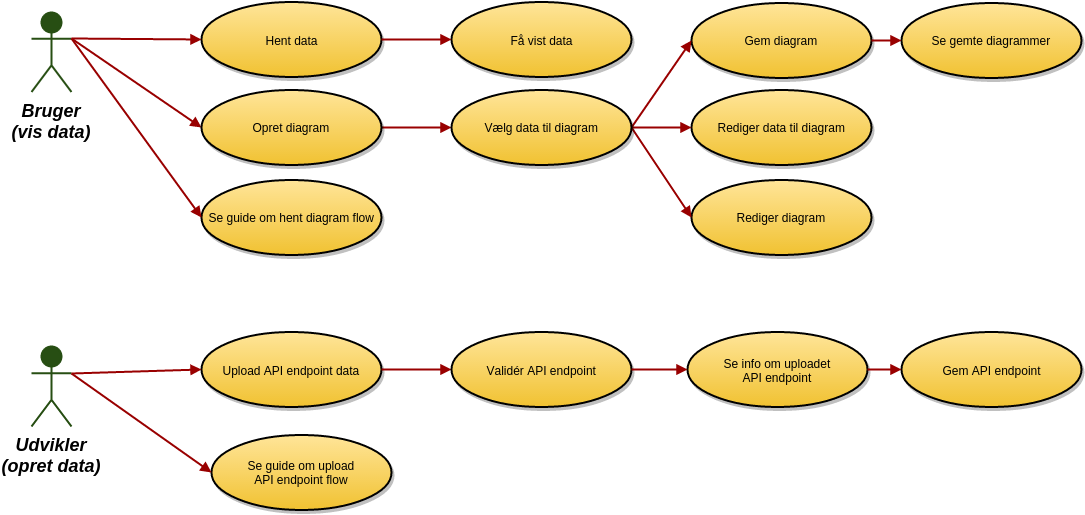
\includegraphics[scale=0.55]{UseCaseDiagram_complete}}
    \caption{Samlet use case diagram}
    \label{fig:usecase-complete}
\end{figure}
\subsection{Use case - Gem API endpoint}
\begin{figure}[H]
    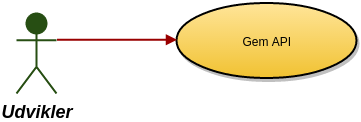
\includegraphics[scale=0.7]{UseCaseDiagram_saveApi}
    \caption{Use case diagram - Gem API endpoint}
    \label{fig:usecase-saveApi}
\end{figure}
\textbf{Aktør:} Udvikler
\\\\
\textbf{Scenarie:} En udvikler vil gemme et API endpoint på vores server da det skal være tilgængeligt i vores system. \\
Brugeren indtaster informationer om sit API endpoint i den givne formular. (Firma, typen af data, url til endpoint). \\
Brugeren modtager herefter en bekræftelse på om data er blevet gemt korrekt.
\\\\
\textbf{Alternative scenarier:} Udvikleren finder det besværligt og får en administrator til at tilføje sit API endpoint,
eller vælger at forlade siden uden at gemme.
